\chapter{Methodology}
\label{methods}
%promises made in other sections:
% * description of disease enrichment method

%intro to the methods


\section{Feature extraction}

Features are the processed form of the data we use to make predictions about a given interaction between pairs of proteins and is defined mathematically in section \ref{supbinclass}.
The process of taking a retrieving these from biological databases is referred to as feature extraction.
This commonly involved mapping between protein identifiers and indexing large tables automatically, but also involved many other small pieces of scripting.

\subsection{Supervised binary classification}
\label{supbinclass}

% going through posing the problem in terms of probability
In supervised learning problems we wish to learn a mapping between input variables and output variables given a training set.
Defining this training set rigorously, it consists of input variables $\pmb{x}$ which are typically vectors of values known as features.
The output variables in a classification problems are a set of labels\autocite[2]{murphy_machine_2012}.
In the case of binary classification these are simply either 0 or 1.
Therefore, given $N$ training vectors $\pmb{x}_{i}$ and training labels $y_{i}$ we can define our training set $\mathcal{D}$ as:

\begin{align}
    \mathcal{D} = \left( ( \pmb{x}_{i}, y_{i} ) \right)_{i=1}^{N}
\end{align}

%an example?

%pose our problem
Our problem involves taking various types of biological data, such as entries from biological databases indicating that proteins are involved in the same part of a cell and using these as features.
The training labels are either an interaction (a one) or a non-interaction (a zero).
Interactions are taken to be any interactions in the HIPPIE\autocite{schaefer_hippie:_2012} database with over 50\% confidence.
Negative interactions are three million random binary combinations of Entrez protein IDs, which is a method applied in other works\autocite{qi_evaluation_2006} to create negative training examples.
There are many more negative that positive interactions and it is unlikely that any of the negative examples are real interactions.

What we would like to estimate is the posterior probability of an interaction existing given a new feature vector after training our classifier.
For a model $\mathcal{H}$ and a new feature vector $\pmb{x}^{*}$ we can express this using Bayes theorem:

\begin{align}
    p(y^{*} = 1 | \pmb{x}^{*}, \mathcal{D}, \mathcal{H}) = \frac{ p(\pmb{x}^{*}| y^{*} = 1 , \mathcal{D}, \mathcal{H}) p( y^{*} = 1 | \mathcal{D}, \mathcal{H})}{ \sum{y^{*}} p( \pmb{x}^{*} | y^{*}, \mathcal{D}, \mathcal{H})}
\end{align}

These expressions are defined:

\begin{itemize}
    \item The posterior probability:
        \begin{align}
            p(y^{*} = 1 | \pmb{x}^{*}, \mathcal{D}, \mathcal{H})
        \end{align}
    \item The likelihood:
        \begin{align}
            p(\pmb{x}^{*}| y^{*} = 1 , \mathcal{D}, \mathcal{H})
        \end{align}
    \item The prior:
        \begin{align}
            p( y^{*} = 1 | \mathcal{D}, \mathcal{H})
        \end{align}
    \item The marginal likelihood:
        \begin{align}
            \sum{y^{*}} p( \pmb{x}^{*} | y^{*}, \mathcal{D}, \mathcal{H})
        \end{align}
\end{itemize}

We do not apply explicitly apply a prior to the probability of interaction, meaning that we implicitly apply a uniform prior.

\subsection{Protein identifier mapping}

Mapping from one protein identifier to another became a significant problem in this project.
Unfortunately, most Biological databases maintain their own indexing method to identify different genes and proteins.
New data sources being integrated into this project would often be using a different identification scheme to that originally chosen to use in PPI network work at Edinburgh: the NCBI Entrez identifier.

%what the Entrez identifier is -  as opposed to other protein identifier schemes - cite NCBI web pages
Genes are defined by their amino acid sequence, but this is a long series of letters and the number of genes is much smaller than the possible combinations of these letters.
For the sake of posterity databases containing information about genes typically apply an identifier for each gene that is much shorter and can encode other information about the gene.
The Entrez GeneID identifier is relatively simple, just consisting of a number generated when the gene was added to the database\autocite{maglott_entrez_2006}.

%other protein identifier schemes and mapping between them
Other popular schemes include the Ensembl identifier from the Ensembl database\autocite{ensembl_website}, Uniprot identifiers from the Uniprot database\autocite{uniprot_website} and even those used only for specific databases such as DIP identifiers\autocite{dip_website}.
Mapping between these different identifiers is difficult as each identifier may map to none or many in another database.
The reason this happens is due to isoforms of different proteins; different amino acid sequences can code for a protein with the same name.


%methods used during the project, with references to appendix notebooks
Various tools exist to map from one protein identifier to another:

\begin{itemize}
    \item Ensembl's BioMart\autocite{smedley_biomart_2009}:
        \begin{itemize}
            \item Able to map from various identifiers to others based on different databases.
            \item Produces a csv which can be used in a variety of different tools.
            \item Requires a list of protein identifiers.
        \end{itemize}
    \item NCBI's Gene\autocite{maglott_entrez_2006} provides conversion tables on it's ftp servers:
        \begin{itemize}
            \item Simple tab-separated text file converting all known GeneIDs between different formats.
        \end{itemize}
    \item The Uniprot\autocite{consortium_universal_2007} online service:
        \begin{itemize}
            \item Similar to BioMart, but with a simpler interface.
            \item Converts only to or from Uniprot identifiers.
            \item Requires a list of protein identifiers.
        \end{itemize}
\end{itemize}

% talk about the problem of canonicalisation
Unfortunately, using any of these services there will be a number of IDs which cannot be converted and many IDs mapping to the same Entrez ID as different protein isoforms are picked up.
One way to avoid this problem is to only refer to a single canonical form of any given protein and find this protein in other databases through its amino acid sequence.
This ensures that when referring to an interaction between two identifiers the interaction is always simply between two proteins.

% how using Entrez identifiers risks becoming gene interaction prediction
% or "What Entrez isn't"
Otherwise, as in this project, the interaction is detected between two Entrez IDs; which corresponds to an interaction between genes - possibly only a single interaction between combinations of the isoforms of each gene.
Unfortunately, this means that this project is only concerned with gene interaction prediction until the Entrez IDs have been carefully canonicalized.
This is not really a problem, as we are only aiming to provide a weighting to a graph, rather than provide an accurate prediction of interaction between proteins.

% how iRefIndex solves this problem and should have been used from the start
% with reference to storing the sequences of each protein involved to maintain unambiguity
A solution to this problem is provided by the iRefIndex\autocite{razick_irefindex_2008} database, which combines many databases and stores canonicalized entries.
Using this database, it would be possible to ensure that the proteins used in a future project would be reliable canonical proteins.
Additionally, each protein of interest should ideally be stored with reference to its sequence in, for example, FASTA format.

%description of feature extraction code
\subsection{Dedicated code: ocbio.extract}



% link to the notebook on using this code
% but update it to explain what custom generator options are

\subsection{Gold standard datasets}
%material on the problems with choosing between gold-standard datasets
% with reference here to the section in Qi's thesis


%original work on DIP (justified choice from previous work)
The database of interacting proteins (DIP) is a database of interactions proven by small-scale experiments\autocite{xenarios_dip_2002}.
Each interaction added is hand curated so it was expected as a reliable training set.
Also, this database was used as a training set in \textcite{qi_evaluation_2006}.

%problems with DIP


%why HIPPIE is better suited

%problem with positive vs. negative ratio with HIPPIE
% and how it's not a problem

%iRefIndex as a final solution?

\subsection{PPI prediction features}

%planned features, describe the list of possible features which was created
%put it in the appendix as a table, or otherwise somehow


%this section should be written with reference to which features were found in the end to be important


%a graph showing the importance of different features is required

%a table describing each feature used, and where it comes from

\subsection{Parallel processing with IPython.parallel}
%description of how this was set up and how it could scale

To take maximum advantage of the available computing facilities and because the sample sizes in the project exceed one million the decision was made to prepare the code for parallel processing on a remote server.
Particularly, grid search operations to optimize performance of the classifier were considered to be processor intensive and vital to the success of the prediction task.
The easiest way to set up these interactive parallel processing operations was the parallel processing model in IPython\autocite{parallel_python_webpage}.

%How this worked in practice, and the potential
The notebooks using parallel processing are the notebooks on classifier training, which are described in Appendix \ref{app:classtrain}.
This usage depended on code from a parallel processing tutorial\autocite{ogrisel_parallel} to distribute memory to the cores using Numpy's memmap methods.
The code to do this has been integrated into the ocbio module in the project repository and can be used as shown in the notebooks.
Potentially, and as described in the tutorial, this code could be used to run the classifier training on cloud services using Starcluster.

%how it should probably have been done differently
However, the gains from parallel processing were mitigated by trying to run the notebook server on the remote server.
The clusters could have been initialised and the jobs submitted locally to the remote server operating as a cluster, thus taking advantage of all the available resources.
This would also be a better system if the parallel processing were to be scaled up to use other processing clusters.

%details of what classifiers were chosen and about scikit-learning
\section{Weighting Protein Interactions}

%classification as a weighting tool
The classification problem we are solving is different in that we are really trying to obtain a realistic weighting of interactions for use in a PPI network.
Classification is normally concerned about picking a decision threshold to classify examples into categories.
However, in this case the output of our process is the posterior probability of the model given a new example.

%introduce scikit-learn
To produce this output the chosen tool was the Python package Scikit-learn\autocite{pedregosa_scikit-learn:_2011}.
Each classifier implemented in this package has a similar interface allowing modular code to be written.
In addition, this package is actively developed with all the required classifiers having efficient implementations.

\subsection{Classification algorithms}

% explain why we tried the algorithms that we tried
Three classification algorithms were chosen to test on the data:

\begin{itemize}
    \item Logistic regression
    \item Support vector machine (SVM)
    \item Random forest
\end{itemize}

The reasons for choosing these and brief description of each algorithm are given below.

\subsubsection{Hyper-parameters}
%describe the different parameters varied in scikit-learn by name
Each of the Classifiers used has hyper-parameters which will affect its performance.
These hyper-parameters are described in table \ref{tab:hyper} for each of the models used in the project.
The optimal values for these found can be found in section \ref{gridresults}, table \ref{tab:gridresults}.

%table of the different hyper-parameters
\begin{table}
    \centering
    \begin{tabular}{l c c}
        Classifier                                  & Hyper-parameters     & Description \\
        \hline
        Logistic Regression                         & C                         &  Inverse of regularisation strength, the $\alpha$ parameter in section \ref{logreg}. \\
        \multirow{3}{*}{Support Vector Machine}     & kernel                    &  The kernel used. Three options: linear, RBF and polynomial. \\
                                                    & Gamma($\gamma$)           &  Kernel coefficient. \\
                                                    & C                         &  As with Logistic Regression, a penalty parameter. \\
        \multirow{2}{*}{Random Forest}              & N estimators              &  Number of trees used in the forest. \\
                                                    & Max features              &  Number of features considered when looking for splits, part of the problem of finding the best decision at each node described in section \ref{randomforest}. \\
        \multirow{2}{*}{Extremely Randomized Trees} & N estimators              &  As with Random Forest. \\
                                                    & Max features              &  As with Random Forest. \\
    \end{tabular}
    \caption{Summary of the hyper-parameters described in the Scikit-learn\cite{pedregosa_scikit-learn:_2011} documentation to be tuned for each of the models considered.}
    \label{tab:hyper}
\end{table}


\subsubsection{Logistic Regression}
\label{logreg}

%with reference to Murphy
Logistic regression is a linear model being used for classification.
It is equivalent to a linear regression model transformed through a sigmoid function\autocite[376]{murphy_machine_2012}:

\begin{align}
    p(c=1|\pmb{x}) = \sigma(b + \pmb{x}^{T}*\pmb{w})
\end{align}

Where $\pmb{x}$ is the vector of features.
The weights and biases are the parameters of this model, expressed in the above equation as $b$ and $\pmb{w}$.

This divides the points in the dataset by a hyperplane, classifying the points on each side into different classes.
For data that is linearly separable, this produces a classifier that will make no mistakes on the test data.
Unfortunately, the data we are working with is not linearly separable.

%How is it trained?
To find the parameters the log likelihood of this model must be maximised; corresponding to the maximum likelihood solution.
The log likelihood for this model is:

\begin{align}
    L(\pmb{w},b) = \sum_{n=1}^{N} c^{n} \log \sigma(b + \pmb{w}^{T}\pmb{x}^{n}) + (1 - c^{n})\log (1 - \sigma(b + \pmb{w}^{T}\pmb{x}^{n}))
\end{align}

%describe what the C parameter is
Regularisation of the weights represents a prior belief that the weights should not increase without bound.
In a case where the data is linearly separable and where regularisation is not applied the weights will increase without bound to produce extremely confident classifications\autocite[381]{barber_bayesian_2013}.
To stop this from happening we apply a penalty term, $\alpha$, to the size of the weights:

\begin{align}
    L'(\pmb{w},b) = L(\pmb{w},b) - \alpha \pmb{w}^{T}\pmb{w}
\end{align}

Tuning this hyper-parameter is the goal of a grid search when training a Logistic Regression model.

\subsubsection{Support Vector Machines}

%with reference to Murphy
Logistic regression can be generalised to apply kernel functions to the input features to obtain better classifications.
Support Vector Machines exploit this while also applying a different objective function intended to avoid overfitting\autocite[383]{murphy_machine_2012}.
The objective in placing the hyperplane for a Support Vector Machine is a "maximum margin" in that is attempts to maintain the same distance from the closest opposing class points.

%success of these models?
These are often successful classifiers in practice.
Applications include text categorisation, hand-written character recognition, image classification and biosequences analysis\autocite{cristianini_an_2000}.

%describe the hyper-parameters?
The hyper-parameters for a Support Vector Machine control the kernels, along with the regularisation parameter as described for logistic regression in section \ref{logreg}.
Two hyper-parameters which can be tuned during a grid search operation are the degree of polynomial kernels if chosen and the gamma coefficient of the kernels.


\subsubsection{Random Forest}
\label{randomforest}

Random forests operate as a combination of many decision trees.
Decision trees are intuitively simple in that it consists of a series of comparisons arranged in a tree as shown in figure \ref{fig:dectree}.

\begin{figure}
    \centering
    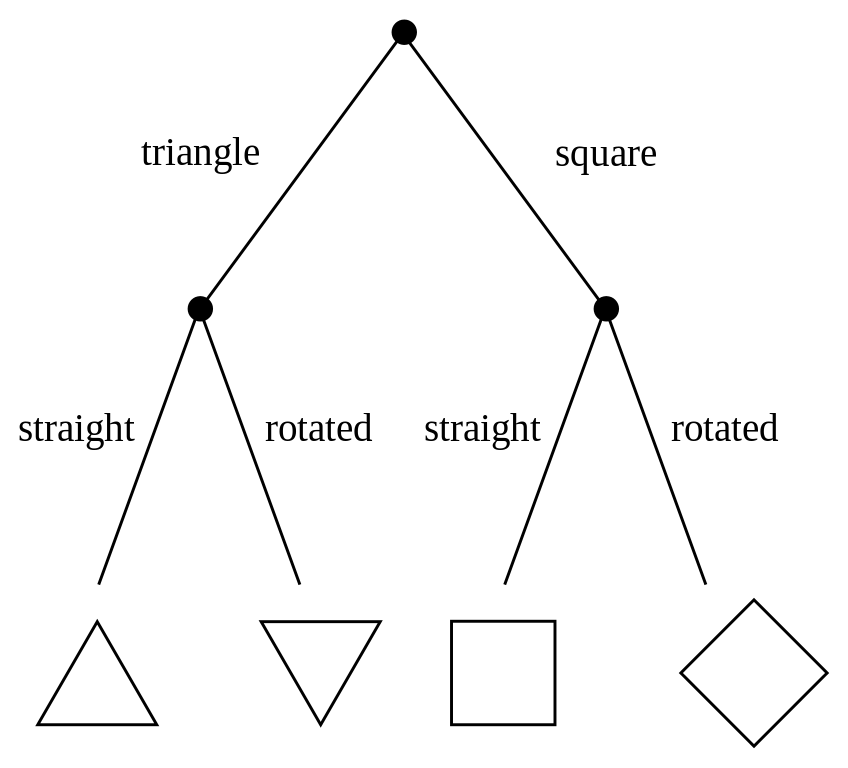
\includegraphics[width=0.8\textwidth]{Simple_decision_tree.png}
    \caption{A simple example decision tree, illustrating the process of sequential, dependent decisions.}
    \label{fig:dectree}
\end{figure}

In this way decision trees are both simple and tractable methods for using a feature vector to classify inputs and there are many automated ways to generate effective decision trees.
The problem in the design of a decision tree is which comparison to choose at each node, described as how to partition the data\autocite[544]{murphy_machine_2012}. %redundant citation here?
There are several implementations of algorithms to achieve this and a full description can be found in \textcite[544]{murphy_machine_2012}.
Other advantages of decision trees include the ability to handle a mixture of discrete and continuous inputs, automatic variable selection, scaling to large datasets readily and the ability to handle missing inputs, with modification.
%other strengths of decision trees?

%describe split function? probably not worth going into this.

%then explain the problems with decision trees, variance etc
Unfortunately, despite the strengths of decision trees there are still problems with stability: small changes in the input data can produce large changes in the output\autocite{murphy_machine_2012}.
The random forest algorithm addresses this problem by providing redundancy; multiple trees are grown and their results averaged.
For M trees trained on different subsets of the data\autocite{murphy_machine_2012}:

\begin{align}
    f(x) = \sum_{m=1}^{M} \frac{1}{M} f_{m}(x)
\end{align}

Where $f_{m}(x)$ is $m$th tree. This is simply averaging the results of the trees and is known as bagging.

%with reference to Qi and ENTS, showing good performance on this problem
With the ability to work on large datasets and mixing continuous and discrete data these types of classifiers would appear to already be well suited to this problem.
This is what has been observed in the literature, with these classifiers achieving the best performance despite different types of biological data being used\autocites{qi_evaluation_2006,rodgers-melnick_predicting_2013}.
Due to these reports in the literature it appeared that this classifier would be the best choice for our protein interaction prediction task.

%expand on how much better they were etc? in different places?

\subsubsection*{Other options}

% what other algorithms could we have tried but didn't
Other options considered for our classification problem, but not included in the project due to time constraints included:

\begin{itemize}
    \item Feedforward neural networks
    \item Naive Bayes
    \item Beta regression
\end{itemize}

Naive Bayes in particular would have required modifying the code from Scikit-learn to deal with data from multiple different distributions or implementing Weka's solution of kernel density estimated distributions for each different feature\autocite{john_estimating_1995}.
Beta regression would have been very suitable for the task and is suggested as future work, described in the following section.

\subsubsection{Beta regression}

%what is beta regression? quickly
A generalised linear model is one in which the output variable is distributed according to a given target density\autocite{murphy_machine_2012}.
In the case of Beta regression\autocite{smithson_better_2006} this target model is the Beta distribution, which has the convenient characteristic of being bounded between 0 and 1.
A maximum-likelihood solution to this model can be found and the resulting model fit in the same way as a standard regression model.

%why this would also have been a good idea, if we didn't have to implement it ourselves
True protein interactions are not something which can be assumed in a protein interaction prediction task.
Many proteins are known to be very likely, but others are less confidently classified, as reflected in the HIPPIE database's confidence scoring system\autocite{schaefer_hippie:_2012}.
To train a classifier a training set of true and false interactions is required and this cannot be supplied without thresholding the database at an arbitrary confidence value.

Beta regression avoids this problem as it allows the confidence values to remain a part of the regression process.
Using this we can build a model and update our belief on the likelihood of interaction in a Bayesian framework much more easily.

\subsection{Classifier verification}
\label{classifierverification}

%Tests we planned to use on each classifier:
%  mention cross-validation
%  learning curves
%  simple accuracy value
%  grid search
%  ROC
%  Precision recall
%  test interactions
%  

% consider using paragraph headings in this section

% was or will be?
Cross-validation was applied to tests during parameters searches and when plotting learning curves to get a statistical estimate of the reliability of the metrics applied to the classifier\autocite[152]{witten_data_2011}.
As the training set is relatively large, these were applied as random sub-samples of the full data set, but stratified to maintain the same proportion of zeros to ones as in the full training set.
This is important as it must reflect the expected ratio for real protein interactions to non-interactions.

\subsubsection{Pipeline}

%what is a pipeline? why did I use one?

\subsubsection{Learning Curves}
% learning curves, what are they? and why?
Learning curves, as in the notebook referenced in Appendix \ref{app:classtrain}, were used in this project to ensure that the number of samples used in a grid search was sufficient.
The learning curve plots the accuracy of a classifier after it has been trained using cross-validation on a varying number of samples.

%example learning curve?


\subsubsection{Grid search}
% grid search
A grid search is a cross-validated test measuring accuracy testing the classifier with a variety of different hyper-parameters.
Classifiers, such as a Logistic Regression model, have some number of hyper-parameters.
A Logistic Regression model, for example, has a single hyper-parameter so that the grid search for this model simply involves varying this parameter to obtain the optimum performance on the test set.

\subsubsection{Accuracy}
% accuracy value
The accuracy value plotted in the learning curve and used in grid searches of parameters values is simply the proportional of correctly classified instances in a training or validation set.
Typically, the protein interaction prediction problem is sparse, in that there are very few interactions for the large number of non-interactions.
This is reflected in the accuracy in that a classifier that simply always predicts zero can still achieve a very high accuracy.
Using this accuracy value is therefore problematic and this requires the other measures employed, such as ROC and precision-recall AUC values.

\subsubsection{ROC curve}
% explain what those are
A Receiver Operating Characteristic, or ROC, curve plots the variation in true positive to false positive rate as the threshold of classification is varied.
This makes it useful as an illustration of the tradeoff possible with this particular classifier.
The Area Under Curve, or AUC, value is the area under this line.
A higher AUC value corresponds to a better classifier, although there is some controversy surrounding this\autocite{hanczar_small-sample_2010}.
These concerns center on the problems of small sample sizes, which are not the case in this project.

\subsubsection{Precision-recall curve}
%precision recall
A precision-recall curve plots the precision of a classifier against its recall as the threshold of classification is varied.
These terms are defined:

\begin{itemize}
    \item Precision - the number of true positive results over the number of total positive results
    \item Recall - the number of true positive results against the number of available positive examples
\end{itemize}

Again, the area under the curve can gauge a classifier's effectiveness.

%example ROC curve?
%example precision recall curve?

\subsection{Missing data}
%how was missing data dealt with?
Before classification could be performed the missing data in the feature vectors had to be imputed.
This was performed by filling the missing values with the mean value of that feature.
This is a common technique that is applied if it is likely the data is missing at random.
In this case the data that is missing is due to mismatches in protein identifier mapping dictionaries, which is likely random and independent of the interaction prediction task.

\subsection{Bayesian weighting}
\label{bayes}

%description of the method used to weight interactions after the classifier was found to be insufficient






\section{Measures applied to weighted and unweighted PPI networks}

%why do we want to try weighted networks? and intro
It is hoped that a weighted graph will provide new insight into the interactions of proteins in the active zone.
For this reason, comparing the unweighted and weighted cases of the graph produced is a major goal of this project.
The following sections describe this process and the measures applied to both graphs.

\subsection{Community detection}

%description of each of the algorithms available
%three:
%  Geodesic edge Betweenness
%  Random edge Betweenness
%  Spectral Betweenness
Three algorithms were identified for use in this project for community detection, the first two are described in \textcite{newman_finding_2004}.
All three are based on betweenness measures to partition the graph, making them optimisation approaches, but each calculates their betweenness measure in a different way:

\begin{itemize}
    \item Geodesic edge betweenness - find the shortest path between all pairs of nodes and count the number of these paths which run along each edge.
    \item Random edge betweenness - expected net number of times that a random walk between two nodes will pass through an edge summed over all node pairs.
    \item Spectral betweenness - pending
\end{itemize}

%community detection code, what it does, which algorithm was used
%pending use - will see if I have time to use more than one

\subsection{Normalised Mutual Information}

%NMI theory, what is a measure of
Mutual information intuitively is the reduction in uncertainty about one random variable by observing another.
Defined in terms of entropy it is\autocite{mackay_information_2003}:

%could move that citation next to the equation?
\begin{align}
    I(X;Y) = H(X) - H(X|Y)
\end{align}

Where $H(X)$ is the entropy of the random variable $X$ and $H(X|Y)$ is the conditional entropy of $X$ given $Y$.

In the case of the function we are using to perform this from Scikit-learn the mutual information is normalised by $\sqrt{H(X)\times H(Y)}$\autocite{pedregosa_scikit-learn:_2011}.
This produces a value between zero and one which reflects the redundancy of the distributions - 1.0 being exactly the same and 0.0 being independent.

Code produced at Edinburgh to calculate NMI was also used.
The problem with the Scikit-learn code is that it assumes the class labels are correct, but they have just been arbitrarily numbered as the communities are found. 
This code takes that into account, ensuring that the class labels are accurate to the IDs in the community.

\subsection{Disease Enrichment}

%Primer on what this test actually does


%interaction between significance level and p-value


\section*{Conclusion}


